\documentclass[12pt, a4paper]{article}
\input{/home/mykhailo/.config/nvim/templates/preamble.tex}

\newcommand{\department}{ЗІ}
\newcommand{\reportnumber}{2}
\newcommand{\reporttitle}{Розмітка вебсторінок за допомогою HTML та за допомогою React}
\newcommand{\profname}{Синявський О. Ю.}

\begin{document}

\input{/home/mykhailo/Documents/lpnu/report_title_page}
\section{Частина 1}
Мета: Ознайомитися з основними принципами розмітки вебсторінок за допомогою HTML. Навчитися правильно створювати структуру HTML-документа (включно з обов'язковими тегами та семантичними розділами), попрактикуватися у використанні базових тегів, атрибутів, блокових та рядкових елементів, а також навчитися користуватися розподіленою системою контролю версій --- Git.
\subsection{Хід роботи}
\begin{enumerate}
	\item \textbf{Підготуйте робоче місце:}
		\begin{itemize}
			\item Створіть окрему папку для цієї лабораторної роботи з назвою \verb|lab_2| на вашому комп'ютері.
			\item Відкрийте цю папку у вашому редакторі коду (наприклад, VS Code).
		\end{itemize}
	\item \textbf{Ініціалізуйте Git-репозиторій:}
		\begin{itemize}
			\item Відкрийте термінал у вашому редакторі або операційній системі
			\item Перейдіть до вашої папки \verb|lab_2|, якщо ви ще не там.
			\item Виконайте команду \verb|git init|.
		\end{itemize}
	\item \textbf{Створіть HTML-файл:}
		\begin{itemize}
			\item Створіть файл з назвою \verb|index.html|.
		\end{itemize}
	\item \textbf{Додайте зміни до відстежуваних (Stage):}
		\begin{itemize}
			\item Виконайте команду \verb|git add index.html|.
		\end{itemize}
	\item \textbf{Напишіть ваш HTML-код:}
		\begin{itemize}
			\item У файлі \verb|index.html| напишіть інформацію про себе та ваш досвід роботи у форматі CV (резюме).
			\item Вимоги:
				\begin{itemize}
					\item Використовуйте семантичні теги HTML.
					\item Використовуйте заголовки, параграфи, списки та посилання.
					\item НЕ використовуйте CSS або JavaScript на цьому етапі. Зосередьтеся виключно на структурі.
				\end{itemize}
		\end{itemize}
	\item \textbf{Зробіть коміт:}
		\begin{itemize}
			\item Виконайте команду \verb|git commit -m "Initial commit of CV structure"|
		\end{itemize}
\end{enumerate}
\subsection{Лістинг}
\small\begin{lstlisting}
<!DOCTYPE html>
<html>
	<head>
		<title>CV - Кохманський Михайло</title>
	</head>
	<body>
		<header>
			<h1>Кохманський Михайло Михайлович</h1>
			<p>Information security specialist</p>
			<p>
				Email: <a href="mailto:mykhailo.kokhmanskyi.kb.2025@lpnu.ua">mykhailo.kokhmanskyi.kb.2025@lpnu.ua</a> |
				GitHub: <a href="https://github.com/MykhailoKokhmanskyi">https://github.com/MykhailoKokhmanskyi</a> | 
				Місто: Львів, Україна
			</p>
		</header>
		<main>
			<section id="about">
				<h2>Про мене</h2>
				<p>
					Я студент спеціальності "Кібербезпека", який захоплюється вивченням методів захисту інформаційних систем, аналізом вразливостей та мережевою безпекою. Активно розвиваю практичні навички в тестуванні на проникнення, безпеці вебдодатків та криптографії, а також регулярно беру участь у CTF-змаганнях. Прагну застосувати отримані знання в реальних проектах для виявлення загрози та побудови надійних систем захисту даних.
				</p>
			</section>
			<section id="education">
				<h2>Освіта</h2>
				<article>
					<h3>F5 - Кібербезпека</h3>
					<p><strong>Національний Університет "Львівська Політехніка"</strong> | <em>2025-2029</em></p>
				</article>
			</section>
			<section id="skills">
				<h2>Навики</h2>
				<ul>
					<li><strong>Мови програмування:</strong> HTML, CSS, JavaScript, Python3, Lua</li>
					<li><strong>Бібліотеки і фреймворки:</strong> React.js, Express.js, Next.js, JWT</li>
					<li><strong>Інструменти</strong> Git, GitHub, Vim, Linux, LaTeX, SQL, MySQL, PostgreSQL, MongoDB, SSL, SSH</li>
				</ul>
			</section>
			<section id="projects">
				<h2>Проекти</h2>
				<article>
					<h3>LPMonitor - Платформа краудсорсингового моніторингу сервісів</h3>
					<p><strong>Технології:</strong> Node.js, Express.js, AWS (Lightsail, SES), HTML, SSR, PostgreSQL</p>
					<p><strong>URL:</strong> <a href="https://lpmonitor.org">https://lpmonitor.org</a>
					<p><strong>Github:</strong> <a href="https://github.com/MykhailoKokhmanskyi/LPMonitor">https://github.com/MykhailoKokhmanskyi/LPMonitor</a>
					<ul>
						<li>Розробив та розгорнув прототип системи моніторингу доступності університетських серввісів на основі краудсорсингу.</li>
						<li>Реалізував базову систему автентифікації користувачів та проміжне програмне забезпечення (middleware) для обробки запитів.</li>
						<li>Налаштував обмеження частоти запитів (Rate Limiting) для захисту сервера від перевантаження та зловживань.</li>
						<li>Налаштував хостинг серверного вебдодатка (SSR) на базі AWS Lightsail, керування DNS-записами та інтегрував AWS SES для надсилання електронних листів для підтвердження електронної адреси.</li>
						<li>Проект відкладено.</li>
					</ul>
				</article>
			</section>
		</main>
		<footer><p>&copy; 2026 Кохманський Михайло. Всі права захищено.</p></footer>
	</body>
</html>
\end{lstlisting}
\subsection{Результат}
\begin{figure}[H]
	\centering
	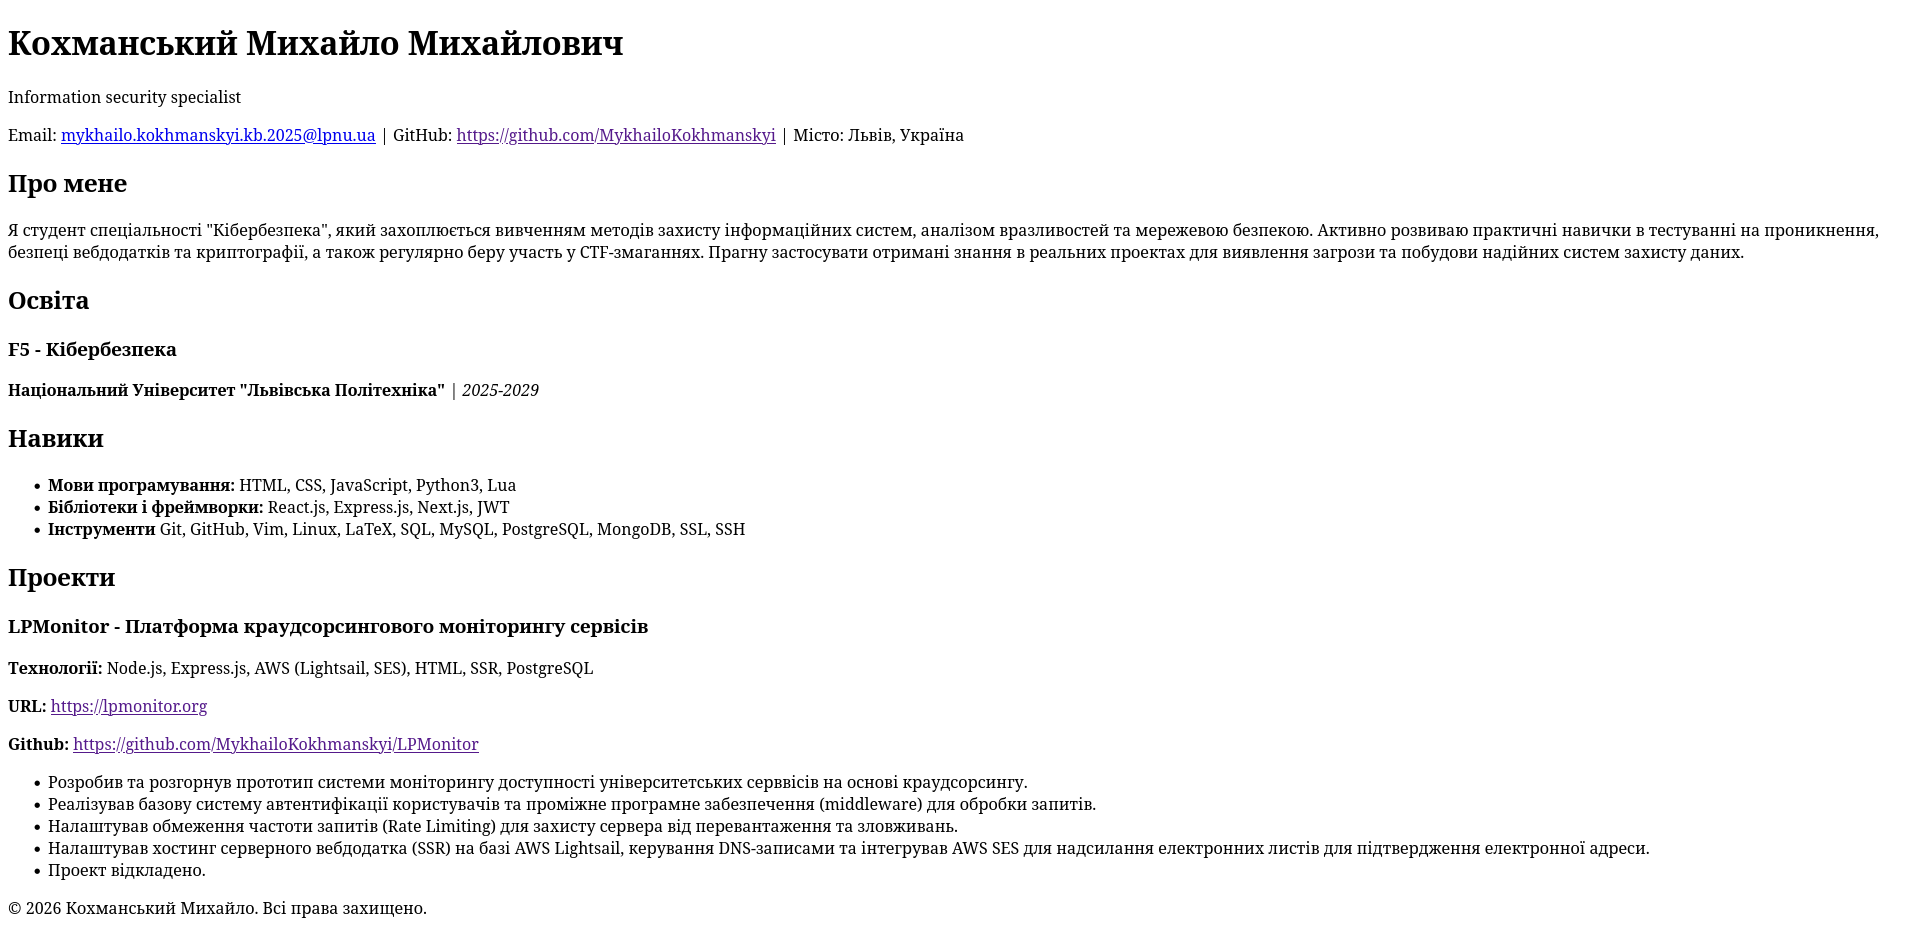
\includegraphics[width=1\textwidth]{appearance.png}
\end{figure}
\section{Частина 2}
Мета: Ознайомитися з основними принципами React та компонентної архітектури. Навчитися створ.вати простий React-застосунок за допомогою Vite. Зрозуміти, як декомпозувати інтерфейс користувача (UI) на компоненти, придатні для повторного використання.
\subsection{Хід роботи}
\begin{enumerate}
	\item \textbf{Ініціалізуйте проєкт:}
		\begin{itemize}
			\item У терміналі переконайтеся, що ви перебуваєте у вашій папці \verb|lab_2|.
			\item Виконайте команду: \verb|npm create vite@latest lab_2_react -- -template reat|.
		\end{itemize}
	\item \textbf{Встановіть залежності:}
		\begin{itemize}
			\item Перейдіть у новостворену папку \verb|cd lab_2_react|.
			\item Виконайте команду \verb|npm install|.
		\end{itemize}
	\item \textbf{Запустіть сервер розробки:}
		\begin{itemize}
			\item Виконайте команду \verb|npm run dev|
			\item Ви повинні побачити URL-адресу. Натисніть на неї з клашівою Command (Mac) або Ctrl (Windows), щоб відкрити її в браузері. Ви повинні побачити сторінку за замовчуванням Vite + React.
		\end{itemize}
	\item \textbf{Встановіть інструменти розробки:}
		\begin{itemize}
			\item Встановіть розширення React Developer Tools для вашого браузера (Chrome, Firefox, або Edge). Це додасть вкладку "Components" до інструментів розробника вашого браузера, що дозволить вам інспектувати компоненти React.
		\end{itemize}
	\item \textbf{Розберіться зі структурою:}
		\begin{itemize}
			\item \verb|src/main.jsx|: Точка входу. Знаходить елемент \verb|root| у вашому HTML і "прикріплює" до нього ваш застосунок React.
			\item \verb|src/App.jsx|: Головний компонент вашого застосунку. Саме тут ви почнете роботу.
		\end{itemize}
	\item \textbf{Створіть свої компоненти:}
		\begin{itemize}
			\item Подивіться на ваше HTML-резюме з Частини 1. Розбийте його на логічні частини.
			\item Завдання: створіть папку \verb|components| всередині \verb|src|.
			\item Створіть нові файли для кожної частини, наприклад: \verb|Header.jsx|, \verb|Experience.jsx|, \verb|Education.jsx|, \verb|Footer.jsx|.
		\end{itemize}
	\item \textbf{Зберіть ваш застосунок:}
		\begin{itemize}
			\item Відкрийте \verb|src/App.jsx|.
			\item Очистіть наявний код всередині функції App
			\item Імпортуйте ваші нові компоненти вгорі файлу.
			\item Використовуйте їх в JSX App.jsx.
		\end{itemize}
	\item \textbf{Перевірте за допомогою DevTools:}
		\begin{itemize}
			\item Відкрийте інструменти розробника у браузері.
			\item Перейдіть на вкладку Components.
			\item Ви повинні побачити деревоподібну структуру
			\item Зробіть скріншот цього дерева компонентів і додайте його до вашого звіту.
		\end{itemize}
	\item \textbf{Зробіть коміт змін:}
		\begin{itemize}
			\item Зупиніть сервер.
			\item Додайте зміни до відстежуваних \verb|git add .|.
			\item Зробіть коміт \verb|git commit -m "Recreated CV using React components"|.
		\end{itemize}
	\item \textbf{Опублікуйте вашу роботу:}
		\begin{itemize}
			\item Cтворіть новий публічний репозиторій на Github.
			\item Дотримуйтесь інструкцій, наданих хостингом, щоб надіслати ваш локальний репозиторій у віддалений.
			\item Скопіюйте посиланння на ваш публічний репозиторій і додайте його до вашого звіту.
		\end{itemize}
\end{enumerate}
\subsection{Результат}
\begin{figure}[H]
	\centering
	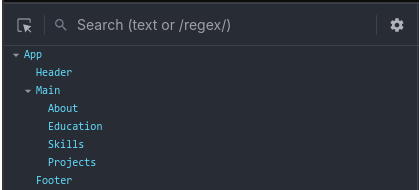
\includegraphics[width=0.5\textwidth]{tree.png}
\end{figure}
Github: \url{https://github.com/MykhailoKokhmanskyi/cybersecurity_web_labs}
\section{Висновок}
Отже, під час виконання цієї лабораторної було ознайомлено з основними принципами розмітки вебсторінок за допомогою HTML. Засвоєно процес правильного створення структури HTML-документа (включно з обов'язковими тегами та семантичними розділами), використання базових тегів, атрибутів, блокових та рядкових елементів, а також користування розподіленою системою контролю версій Git.

Також було засвоєно основні принципи React та компонентрної архітектури, створення простих React-застосунків за допомогою Vite. Опановано навики декомпозиції інтерфейсу користувача на компоненти, придатні для повторного використання.
\end{document}
